% Provenance (never printed): 6e geography and cycle 3 sciences (locating a
% place on the globe: parallels, meridians, latitude, longitude; the Earth's
% rotation and time zones); see sources/book1/PROVENANCE.md.
% Book 1, grade 6, chapter 2.
\chapter{Latitud, longitud y husos horarios}\label{ch:g6:latitude-longitude}

Ha caído la noche sobre el \omterm{def:g2:water-on-earth:ocean}{océano}. En la cubierta de un velero, en el año
1750, el navegante alza su instrumento hacia una estrella brillante y mide
a qué altura está sobre el \omterm{def:g2:water-on-earth:ocean}{mar}. Unos minutos de trabajo, y ya sabe a qué
distancia al norte del \omterm{def:g3:continents-and-oceans:equator}{ecuador} está el barco. Pero ¿a qué distancia al este
o al oeste? Eso no lo puede saber. El problema era tan grave que en 1714 el
Parlamento británico había prometido un gran premio a quien encontrara un
modo de medirlo en el \omterm{def:g2:water-on-earth:ocean}{mar}. Hoy, el teléfono que llevas en el bolsillo da
las dos respuestas en un segundo.
% ledger: rmg:15deg-per-hour, rmg:longitude-act-1714

\begin{omfigure}
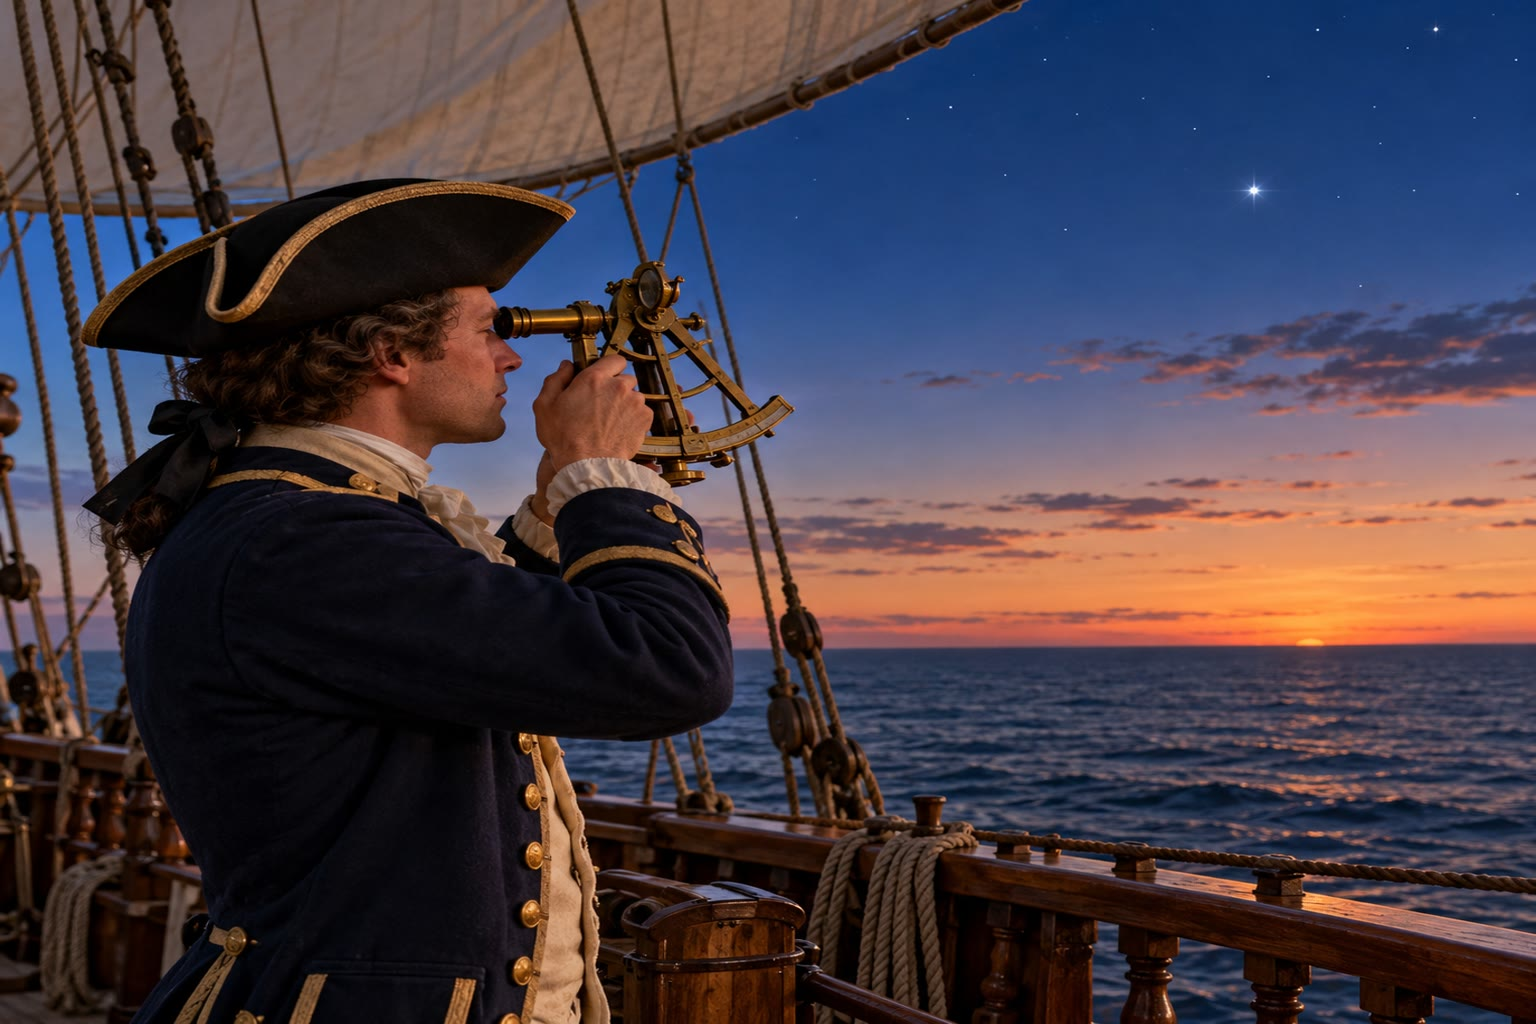
\includegraphics[width=0.62\linewidth]{images/book1/ai/g6-navigator-sextant.jpg}

{\small Un navegante del siglo~XVIII mide la altura de una estrella sobre
el horizonte del \omterm{def:g2:water-on-earth:ocean}{mar}. (Ilustración generada por IA.)}
\end{omfigure}

\begin{recall}
Un \omterm{def:g3:continents-and-oceans:globe}{globo terráqueo} es una pequeña maqueta de la Tierra. El \omterm{def:g3:continents-and-oceans:equator}{ecuador} es la
línea que da la vuelta al \omterm{def:g3:continents-and-oceans:globe}{globo} por el medio, a mitad de camino entre el
\omterm{def:g3:continents-and-oceans:poles}{Polo Norte} y el \omterm{def:g3:continents-and-oceans:poles}{Polo Sur}; corta la Tierra en el \omterm{def:g3:continents-and-oceans:equator}{hemisferio norte} y el
\omterm{def:g3:continents-and-oceans:equator}{hemisferio sur} (\cref{ch:g3:continents-and-oceans}). Los libros de física
mostraron que la Tierra gira sobre sí misma alrededor de un eje que pasa
por los dos \omterm{def:g3:continents-and-oceans:poles}{polos}, una vez al día: este giro trae el día y la noche.
\end{recall}

\section{Los paralelos y la latitud}

Para decir dónde está un lugar de la Tierra, necesitamos dos números, como
la fila y la columna de una butaca en un cine. El primero dice a qué
distancia al norte o al sur del \omterm{def:g3:continents-and-oceans:equator}{ecuador} está el lugar.

Imagina la Tierra cortada en dos, por los dos \omterm{def:g3:continents-and-oceans:poles}{polos}, como una manzana
cortada de arriba abajo desde el rabito. En la cara del corte (abajo, a la
izquierda), el \omterm{def:g3:continents-and-oceans:equator}{ecuador} es la línea horizontal que pasa por el centro. Un
lugar~P de la superficie se ve desde el centro con un cierto ángulo por
encima o por debajo de esa línea: ese ángulo es su \omterm{def:g6:latitude-longitude:latitude}{latitud}.

\begin{omfigure}
\begin{minipage}[t]{0.48\linewidth}\centering
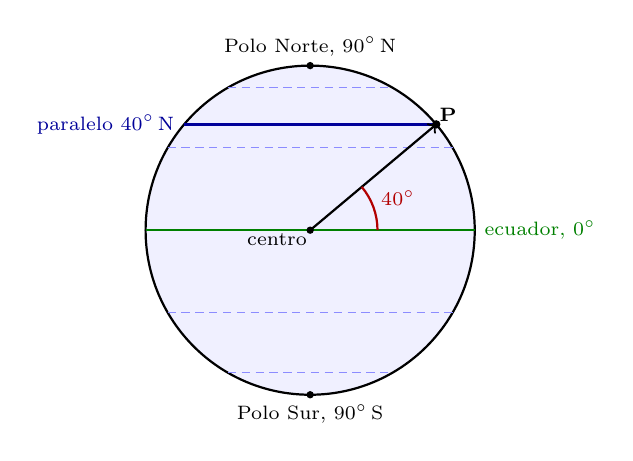
\begin{tikzpicture}[scale=0.95]
  \def\R{2.2}
  \fill[blue!6] (0,0) circle (\R);
  \draw[thick] (0,0) circle (\R);
  % parallels seen edge-on: horizontal chords
  \foreach \a in {-60,-30,30,60}{
    \draw[blue!45, densely dashed] ({-\R*cos(\a)},{\R*sin(\a)}) -- ({\R*cos(\a)},{\R*sin(\a)});}
    \draw[green!50!black, thick] (-\R,0) -- (\R,0);
  \node[font=\scriptsize, green!50!black, anchor=west] at (\R,0) {ecuador, $0^\circ$};
  \draw[blue!60!black, thick] ({-\R*cos(40)},{\R*sin(40)}) -- ({\R*cos(40)},{\R*sin(40)});
  \draw[->, thick] (0,0) -- ({\R*cos(40)},{\R*sin(40)});
  \fill (0,0) circle (1.4pt) node[below left, font=\scriptsize, inner sep=1pt] {centro};
  \fill ({\R*cos(40)},{\R*sin(40)}) circle (1.6pt)
    node[above right, font=\scriptsize\bfseries, inner sep=1pt] {P};
  \draw[red!70!black, thick] (0.9,0) arc (0:40:0.9);
  \node[red!70!black, font=\scriptsize] at (20:1.25) {$40^\circ$};
  \node[font=\scriptsize, blue!60!black, anchor=east] at ({-\R*cos(40)},{\R*sin(40)}) {paralelo $40^\circ$\,N};
  \fill (0,\R) circle (1.4pt) node[above, font=\scriptsize] {Polo Norte, $90^\circ$\,N};
  \fill (0,-\R) circle (1.4pt) node[below, font=\scriptsize] {Polo Sur, $90^\circ$\,S};
\end{tikzpicture}

{\small La \omterm{def:g6:latitude-longitude:latitude}{latitud}: el ángulo en el centro de la Tierra entre el \omterm{def:g3:continents-and-oceans:equator}{ecuador} y
el lugar.}
\end{minipage}\hfill
\begin{minipage}[t]{0.48\linewidth}\centering
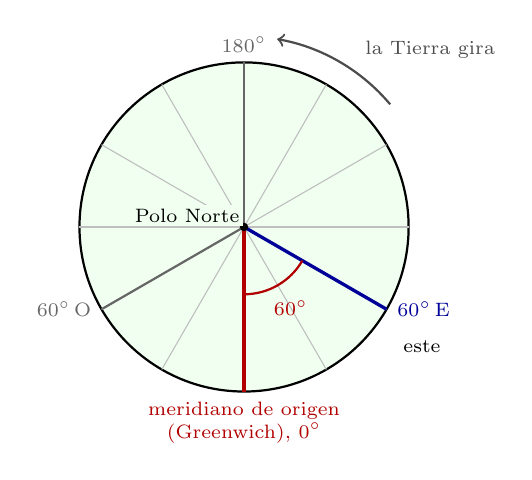
\begin{tikzpicture}[scale=0.95]
  \def\R{2.2}
  \fill[green!6] (0,0) circle (\R);
  \draw[thick] (0,0) circle (\R);
  \foreach \a in {0,30,...,330}{\draw[black!25] (0,0) -- (\a:\R);}
    \draw[red!70!black, very thick] (0,0) -- (270:\R)
    node[below, font=\scriptsize, align=center] {meridiano de origen\\(Greenwich), $0^\circ$};
  \draw[blue!60!black, very thick] (0,0) -- (330:\R)
    node[right, font=\scriptsize] {$60^\circ$\,E};
  \draw[black!60, thick] (0,0) -- (210:\R) node[left, font=\scriptsize] {$60^\circ$\,O};
  \draw[black!60, thick] (0,0) -- (90:\R) node[above, font=\scriptsize] {$180^\circ$};
  \draw[red!70!black, thick] (270:0.9) arc (270:330:0.9);
  \node[red!70!black, font=\scriptsize] at (300:1.25) {$60^\circ$};
    \fill (0,0) circle (1.6pt) node[above left, font=\scriptsize, inner sep=1.5pt, fill=green!6] {Polo Norte};
  \draw[->, thick, black!70] (40:2.55) arc (40:80:2.55);
  \node[font=\scriptsize, black!70, anchor=south west] at (55:2.6) {la Tierra gira};
  \node[font=\scriptsize, anchor=west] at (2.0,-1.6) {este $\circlearrowleft$};
\end{tikzpicture}

{\small La \omterm{def:g6:latitude-longitude:longitude}{longitud}: la Tierra vista desde encima del \omterm{def:g3:continents-and-oceans:poles}{Polo Norte}. El ángulo
se mide desde el \omterm{def:g6:latitude-longitude:longitude}{meridiano de origen}, hacia el este o hacia el oeste.}
\end{minipage}
% ledger: rmg:latitude-def, rmg:longitude-def
\end{omfigure}

\begin{definition}[Paralelo y latitud]\label{def:g6:latitude-longitude:latitude}
Un \emph{paralelo}\index{paralelo} es un círculo trazado alrededor del \omterm{def:g3:continents-and-oceans:globe}{globo}
paralelo al \omterm{def:g3:continents-and-oceans:equator}{ecuador}; todos los lugares de un mismo paralelo están a la misma
distancia del \omterm{def:g3:continents-and-oceans:equator}{ecuador}. La \emph{latitud}\index{latitud} de un lugar es el
ángulo, medido en el centro de la Tierra, entre el \omterm{def:g3:continents-and-oceans:equator}{ecuador} y ese lugar. Va
de $0^\circ$ en el \omterm{def:g3:continents-and-oceans:equator}{ecuador} a $90^\circ$ en los \omterm{def:g3:continents-and-oceans:poles}{polos}, y decimos si el lugar
está al norte (N) o al sur (S) del \omterm{def:g3:continents-and-oceans:equator}{ecuador}.
% ledger: rmg:latitude-def
\end{definition}

El propio \omterm{def:g3:continents-and-oceans:equator}{ecuador} es un \omterm{def:g6:latitude-longitude:latitude}{paralelo}, el más largo, de \omterm{def:g6:latitude-longitude:latitude}{latitud} $0^\circ$. Los
\omterm{def:g6:latitude-longitude:latitude}{paralelos} se acortan hacia los \omterm{def:g3:continents-and-oceans:poles}{polos}, y cada \omterm{def:g3:continents-and-oceans:poles}{polo} es un solo punto, a
$90^\circ$\,N o a $90^\circ$\,S. A lo largo de una línea que va de un \omterm{def:g3:continents-and-oceans:poles}{polo}
al \omterm{def:g3:continents-and-oceans:equator}{ecuador}, cada grado de \omterm{def:g6:latitude-longitude:latitude}{latitud} mide unos \qty{111}{km}.
% ledger: rmg:latitude-def

La \omterm{def:g6:latitude-longitude:latitude}{latitud} es el número fácil: se puede encontrar en el cielo. De día, los
marinos medían la altura del Sol a mediodía; de noche, en el \omterm{def:g3:continents-and-oceans:equator}{hemisferio
norte}, medían la altura de la Estrella Polar. Es lo que hace el navegante
de la imagen del principio.
% ledger: rmg:15deg-per-hour

La Estrella Polar está casi exactamente sobre la línea del eje de la
Tierra, prolongada más allá del \omterm{def:g3:continents-and-oceans:poles}{Polo Norte}, y tan lejos que su luz llega a
todos los lugares de la Tierra en líneas paralelas. En el \omterm{def:g3:continents-and-oceans:poles}{Polo Norte} está
justo en lo alto, a $90^\circ$ sobre el horizonte; en el \omterm{def:g3:continents-and-oceans:equator}{ecuador} está sobre
el horizonte norte, a $0^\circ$. Entre los dos, la regla es sencilla:
\emph{la altura de la Estrella Polar sobre el horizonte norte, medida como
un ángulo, es igual a la \omterm{def:g6:latitude-longitude:latitude}{latitud}}. La figura de abajo muestra por qué los
dos ángulos son iguales.
% ledger: nsta:polaris-latitude

\begin{omfigure}
\begin{tikzpicture}[scale=1.1, font=\scriptsize]
  \def\R{1.7}
  \coordinate (O) at (0,0);
  \coordinate (P) at ({\R*cos(40)},{\R*sin(40)});
  \fill[blue!8] (O) circle (\R);
  \draw[black!70] (O) circle (\R);
  % equator and axis
  \draw[black!50] (-\R,0) -- (\R,0);
  \node[black!60, anchor=north east] at (-0.15,0) {ecuador};
  \draw[black!70, -{Stealth[length=2mm]}] (0,-\R-0.3) -- (0,\R+1.7);
  \node[anchor=east, align=right] at (-0.1,\R+1.45) {hacia la Estrella Polar\\(muy lejos)};
  \node[anchor=south east] at (0,\R) {N};
  % radius to P and latitude angle at the centre
  \draw[black!80] (O) -- (P);
  \draw[red!70!black, thick] (0.55,0) arc (0:40:0.55);
  \node[red!70!black] at (20:0.8) {$40^\circ$};
  % horizon at P (tangent) and the ray to the Pole Star (parallel to the axis)
  \draw[black!70, thick] ($(P)+({-sin(40)*1.5},{cos(40)*1.5})$) -- ($(P)+({sin(40)*1.6},{-cos(40)*1.6})$);
  \node[anchor=south, rotate=-50, inner sep=2pt] at ($(P)+({sin(40)*1.15},{-cos(40)*1.15})$) {horizonte};
  \draw[orange!80!black, thick, -{Stealth[length=2mm]}] (P) -- ++(0,1.45);
  \draw[red!70!black, thick] ($(P)+(0,0.7)$) arc (90:130:0.7);
  \node[red!70!black] at ($(P)+(110:0.98)$) {$40^\circ$};
  \fill (P) circle (1.4pt);
  \node[anchor=west] at ($(P)+(0.3,0.05)$) {observador a $40^\circ$\,N};
\end{tikzpicture}

{\small Por qué la altura de la Estrella Polar es igual a la \omterm{def:g6:latitude-longitude:latitude}{latitud} (un
esquema, no a escala). La luz de la Estrella Polar llega paralela al eje de
la Tierra (en naranja). El horizonte del observador forma un ángulo recto
con el radio que pasa por el observador; el eje forma un ángulo recto con
el \omterm{def:g3:continents-and-oceans:equator}{ecuador}. Así que el ángulo
entre el horizonte y la Estrella Polar es igual a la \omterm{def:g6:latitude-longitude:latitude}{latitud}, el ángulo en
el centro entre el \omterm{def:g3:continents-and-oceans:equator}{ecuador} y el observador.}
% ledger: nsta:polaris-latitude
\end{omfigure}

\begin{example}[Una navegante de noche]\label{ex:g6:latitude-longitude:pole-star}
Una navegante mide la Estrella Polar a $41^\circ$ sobre el horizonte norte.
El barco está a la \omterm{def:g6:latitude-longitude:latitude}{latitud} $41^\circ$\,N, a unos $41 \times 111
\approx \num{4550}$~km al norte del \omterm{def:g3:continents-and-oceans:equator}{ecuador}. Navegando hacia el norte, ve la
estrella un poco más alta cada noche; navegando hacia el sur, hacia el
\omterm{def:g3:continents-and-oceans:equator}{ecuador}, la estrella baja hacia el horizonte. Al sur del \omterm{def:g3:continents-and-oceans:equator}{ecuador} la
Estrella Polar no se ve en absoluto, porque se queda bajo el horizonte:
allí, el Sol del mediodía da la \omterm{def:g6:latitude-longitude:latitude}{latitud}.
\end{example}
% ledger: nsta:polaris-latitude, rmg:latitude-def, rmg:15deg-per-hour

\section{Los meridianos y la longitud}

El segundo número dice a qué distancia al este o al oeste está un lugar.
Aquí no hay una línea de partida natural como el \omterm{def:g3:continents-and-oceans:equator}{ecuador}: hay que elegirla.

\begin{definition}[Meridiano, longitud y meridiano de origen]\label{def:g6:latitude-longitude:longitude}
Un \emph{meridiano}\index{meridiano} es un semicírculo trazado sobre el
\omterm{def:g3:continents-and-oceans:globe}{globo} desde el \omterm{def:g3:continents-and-oceans:poles}{Polo Norte} hasta el \omterm{def:g3:continents-and-oceans:poles}{Polo Sur}. El \emph{meridiano de
origen}\index{meridiano de origen} es el meridiano elegido como línea de
partida: el que pasa por el antiguo Real Observatorio de Greenwich, en
Londres. La \emph{longitud}\index{longitud} de un lugar es el ángulo entre
el meridiano de origen y el meridiano de ese lugar, visto desde el eje de
la Tierra. Va de $0^\circ$ en el meridiano de origen a $180^\circ$, y
decimos si el lugar está al este (E) o al oeste (O) del meridiano de
origen.
% ledger: rmg:longitude-def
\end{definition}

Todos los \omterm{def:g6:latitude-longitude:longitude}{meridianos} se juntan en los \omterm{def:g3:continents-and-oceans:poles}{polos}, y todos tienen la misma
\omterm{def:g6:latitude-longitude:longitude}{longitud}. En el lado de la Tierra opuesto a Greenwich, el \omterm{def:g6:latitude-longitude:longitude}{meridiano}
$180^\circ$\,E y el \omterm{def:g6:latitude-longitude:longitude}{meridiano} $180^\circ$\,O son la misma línea.

\begin{omfigure}
\begin{minipage}[c]{0.46\linewidth}\centering
\begin{tikzpicture}
  \begin{axis}[axis equal image, hide axis, width=\linewidth,
      xmin=-1.05, xmax=1.05, ymin=-1.05, ymax=1.12, clip=false]
    \fill[omSea] (axis cs:0,0) circle (1);
    \addplot[fill=omLithAlluv, draw=black!45, line width=0.2pt] table {figdata/out/grade-6-graticule-land.dat};
    \addplot[blue!50!black, line width=0.35pt] table {figdata/out/grade-6-graticule-parallels.dat};
    \addplot[black!55, line width=0.35pt] table {figdata/out/grade-6-graticule-meridians.dat};
        \addplot[green!50!black, line width=1.1pt] table {figdata/out/grade-6-graticule-equator.dat};
    \addplot[red!70!black, line width=1.1pt] table {figdata/out/grade-6-graticule-prime.dat};
    \draw[black!70] (axis cs:0,0) circle (1);
    \fill (axis cs:0,0.9063) circle (1.3pt);
        \node[font=\scriptsize, above left, inner sep=1.5pt] at (axis cs:0,0.9063) {N};
  \end{axis}
\end{tikzpicture}
\end{minipage}\hfill
\begin{minipage}[c]{0.5\linewidth}
{\small Un \omterm{def:g3:continents-and-oceans:globe}{globo} con sus \omterm{def:g6:latitude-longitude:latitude}{paralelos} (en azul) y sus \omterm{def:g6:latitude-longitude:longitude}{meridianos} (en gris),
cada $30^\circ$. El \omterm{def:g3:continents-and-oceans:equator}{ecuador} está dibujado en verde grueso, y el \omterm{def:g6:latitude-longitude:longitude}{meridiano
de origen}, en rojo; se cruzan en el \omterm{def:g2:water-on-earth:ocean}{océano}, al sur de Ghana, en la \omterm{def:g6:latitude-longitude:latitude}{latitud}
$0^\circ$ y la \omterm{def:g6:latitude-longitude:longitude}{longitud} $0^\circ$. Cada \omterm{def:g6:latitude-longitude:longitude}{meridiano} va de \omterm{def:g3:continents-and-oceans:poles}{polo} a \omterm{def:g3:continents-and-oceans:poles}{polo}; cada
\omterm{def:g6:latitude-longitude:latitude}{paralelo} es un círculo alrededor del eje. (Tierras: Natural Earth.)}
% ledger: data:ne-land (figdata/grade-6/graticule.py)
\end{minipage}
\end{omfigure}

\begin{history}[La elección del meridiano de origen]
Durante mucho tiempo, cada país dibujó sus \omterm{def:g2:drawing-to-map:map}{mapas} con su propio \omterm{def:g6:latitude-longitude:longitude}{meridiano} de
partida: se usaron Londres, París y otros lugares. En octubre de 1884,
delegados de muchos países se reunieron en Washington para elegir un solo
\omterm{def:g6:latitude-longitude:longitude}{meridiano} para todo el mundo. El 13~de octubre votaron proponer el
\omterm{def:g6:latitude-longitude:longitude}{meridiano} que pasa por el observatorio de Greenwich: 21 países votaron a
favor, uno en contra y dos no votaron.
% ledger: rmg:longitude-def, meridian:1884-vote
\end{history}

\section{Encontrar un lugar por sus dos ángulos}

Con su \omterm{def:g6:latitude-longitude:latitude}{latitud} y su \omterm{def:g6:latitude-longitude:longitude}{longitud}, cualquier lugar de la Tierra se puede
encontrar en un \omterm{def:g2:drawing-to-map:map}{mapa} o en un \omterm{def:g3:continents-and-oceans:globe}{globo}. Escribimos primero la \omterm{def:g6:latitude-longitude:latitude}{latitud}: El
Cairo, por ejemplo, está a unos $30^\circ$\,N, $31^\circ$\,E.
% ledger: data:b1-ne-places (figdata/grade-6/cities.py)

\begin{omfigure}
\begin{tikzpicture}
  \begin{axis}[ommap, width=\linewidth,
      xtick={-180,-150,...,180}, ytick={-90,-60,...,90},
      xticklabels={$180^\circ$,$150^\circ$O,$120^\circ$O,$90^\circ$O,$60^\circ$O,$30^\circ$O,$0^\circ$,
                   $30^\circ$E,$60^\circ$E,$90^\circ$E,$120^\circ$E,$150^\circ$E,$180^\circ$},
      yticklabels={$90^\circ$S,$60^\circ$S,$30^\circ$S,$0^\circ$,$30^\circ$N,$60^\circ$N,$90^\circ$N},
      tick label style={font=\tiny}, grid style={black!35, line width=0.3pt}]
    \addplot[fill=omLithAlluv, draw=black!45, line width=0.2pt] table {figdata/out/shared-geo-land.dat};
        \draw[green!50!black, line width=0.9pt] (axis cs:-180,0) -- (axis cs:180,0);
    \draw[red!70!black, line width=0.9pt] (axis cs:0,-90) -- (axis cs:0,90);
    \addplot[only marks, mark=*, mark size=1.2pt, black]
      table[x=lon, y=lat] {figdata/out/grade-6-cities-map.dat};
    % the city names of figdata/out/grade-6-cities-map.dat, written here in Spanish
    \node[font=\tiny, inner sep=1.2pt, anchor=south, fill=white, fill opacity=0.75, text opacity=1] at (axis cs:-21.936,64.144) {Reikiavik};
    \node[font=\tiny, inner sep=1.2pt, anchor=south, fill=white, fill opacity=0.75, text opacity=1] at (axis cs:-0.119,51.502) {Londres};
    \node[font=\tiny, inner sep=1.2pt, anchor=west, fill=white, fill opacity=0.75, text opacity=1] at (axis cs:-73.996,40.722) {Nueva~York};
    \node[font=\tiny, inner sep=1.2pt, anchor=east, fill=white, fill opacity=0.75, text opacity=1] at (axis cs:-118.232,34.049) {Los~Ángeles};
    \node[font=\tiny, inner sep=1.2pt, anchor=east, fill=white, fill opacity=0.75, text opacity=1] at (axis cs:-78.502,-0.213) {Quito};
    \node[font=\tiny, inner sep=1.2pt, anchor=west, fill=white, fill opacity=0.75, text opacity=1] at (axis cs:-43.212,-22.907) {Río~de~Janeiro};
    \node[font=\tiny, inner sep=1.2pt, anchor=north, fill=white, fill opacity=0.75, text opacity=1] at (axis cs:18.433,-33.918) {Ciudad~del~Cabo};
    \node[font=\tiny, inner sep=1.2pt, anchor=west, fill=white, fill opacity=0.75, text opacity=1] at (axis cs:36.815,-1.281) {Nairobi};
    \node[font=\tiny, inner sep=1.2pt, anchor=south, fill=white, fill opacity=0.75, text opacity=1] at (axis cs:31.248,30.052) {El~Cairo};
    \node[font=\tiny, inner sep=1.2pt, anchor=north, fill=white, fill opacity=0.75, text opacity=1] at (axis cs:72.876,19.068) {Bombay};
    \node[font=\tiny, inner sep=1.2pt, anchor=west, fill=white, fill opacity=0.75, text opacity=1] at (axis cs:139.75,35.687) {Tokio};
    \node[font=\tiny, inner sep=1.2pt, anchor=south, fill=white, fill opacity=0.75, text opacity=1] at (axis cs:151.213,-33.871) {Sídney};
    \node[font=\tiny, inner sep=1.2pt, anchor=north east, fill=white, fill opacity=0.75, text opacity=1] at (axis cs:174.763,-36.848) {Auckland};
  \end{axis}
\end{tikzpicture}

{\small Trece ciudades en un \omterm{def:g3:continents-and-oceans:world-map}{mapamundi} con una cuadrícula cada $30^\circ$.
El \omterm{def:g3:continents-and-oceans:equator}{ecuador} está dibujado en verde, y el \omterm{def:g6:latitude-longitude:longitude}{meridiano de origen}, en rojo.
(\omterm{def:g1:landscapes-around-us:water}{Costas} y ciudades: Natural Earth.)}
% ledger: data:ne-land, data:b1-ne-places (figdata/grade-6/cities.py, part map)
\end{omfigure}

\begin{method}[Situar un lugar por sus coordenadas]\label{met:g6:latitude-longitude:locating}
\begin{enumerate}
  \item \omterm{def:g6:latitude-longitude:latitude}{Latitud}: parte del \omterm{def:g3:continents-and-oceans:equator}{ecuador} y ve hacia el norte (N) o hacia el sur
        (S), contando los \omterm{def:g6:latitude-longitude:latitude}{paralelos}, hasta el número de grados correcto.
  \item Longitud: parte del \omterm{def:g6:latitude-longitude:longitude}{meridiano de origen} y ve hacia el este (E) o
        hacia el oeste (O), contando los \omterm{def:g6:latitude-longitude:longitude}{meridianos}, hasta el número de
        grados correcto.
  \item El lugar está donde se cruzan el \omterm{def:g6:latitude-longitude:latitude}{paralelo} y el \omterm{def:g6:latitude-longitude:longitude}{meridiano}. Entre dos
        líneas de la cuadrícula, haz una estimación: a mitad de camino entre
        $30^\circ$ y $60^\circ$ está $45^\circ$.
\end{enumerate}
\end{method}

\begin{example}[Leer las coordenadas de Sídney]\label{ex:g6:latitude-longitude:sydney}
En el \omterm{def:g2:drawing-to-map:map}{mapa}, Sídney está por debajo del \omterm{def:g3:continents-and-oceans:equator}{ecuador}: está en el \omterm{def:g3:continents-and-oceans:equator}{hemisferio sur},
un poco por encima del \omterm{def:g6:latitude-longitude:latitude}{paralelo} $30^\circ$\,S, más cerca de $30^\circ$
que de $60^\circ$; su \omterm{def:g6:latitude-longitude:latitude}{latitud} es de unos $34^\circ$\,S. Está a la derecha
del \omterm{def:g6:latitude-longitude:longitude}{meridiano de origen}, un poco más allá del \omterm{def:g6:latitude-longitude:longitude}{meridiano} $150^\circ$\,E; su
\omterm{def:g6:latitude-longitude:longitude}{longitud} es de unos $151^\circ$\,E. Escribimos: Sídney, $34^\circ$\,S,
$151^\circ$\,E.
% ledger: data:b1-ne-places (cities.py: 33.87 S, 151.21 E)
\end{example}

\section{La Tierra que gira y los husos horarios}

La Tierra gira sobre sí misma una vez al día, de oeste a este. Al girar, el
Sol parece cruzar el cielo de este a oeste. Cuando el Sol está en lo más
alto del cielo, es mediodía. Pero no es mediodía en todas partes en el
mismo momento: cuando es mediodía en Londres, en El Cairo, más al este, ya
es por la tarde, y en Nueva York, más al oeste, todavía es por la mañana.

¿Cuánto gira la Tierra en una hora? Una vuelta completa son $360^\circ$, y
tarda 24~horas:
\[
360^\circ \div 24 = 15^\circ \text{ por hora.}
\]
Así que dos lugares separados por $15^\circ$ de \omterm{def:g6:latitude-longitude:longitude}{longitud} tienen su mediodía
con una hora de diferencia: el lugar más al este lo tiene primero. Un grado
lleva 4~minutos.
% ledger: planet:Earth.day, rmg:15deg-per-hour

\begin{definition}[Huso horario]\label{def:g6:latitude-longitude:time-zone}
Un \emph{huso horario}\index{huso horario} es una franja de la Tierra, de
\omterm{def:g3:continents-and-oceans:poles}{polo} a \omterm{def:g3:continents-and-oceans:poles}{polo}, en la que todos los relojes marcan la misma hora. Idealmente,
cada huso tiene $15^\circ$ de \omterm{def:g6:latitude-longitude:longitude}{longitud} de ancho, de modo que hay 24 husos,
uno por cada hora; al pasar a un huso hacia el este, los relojes marcan una
hora más.
\end{definition}

En los husos ideales, el huso de un lugar es su \omterm{def:g6:latitude-longitude:longitude}{longitud} dividida entre
$15$, redondeada al número entero más cercano: al este de Greenwich sumamos
esas horas a la hora de Greenwich, y al oeste las restamos. Tokio, a
$140^\circ$\,E: $140 \div 15 \approx 9.3$, así que el huso es $+9$: cuando
es mediodía en Greenwich, son las 9 de la noche en Tokio. Los \omterm{def:g6:latitude-longitude:time-zone}{husos
horarios} reales no son franjas rectas: siguen las fronteras de los países
y de las regiones, para que todo un país, o toda una región, tenga la misma
hora.
% ledger: data:b1-ne-places, rmg:15deg-per-hour

\begin{omfigure}
\begin{tikzpicture}
  \begin{axis}[ommap, width=\linewidth, clip=false,
      xtick={-180,-90,0,90,180}, ytick={-60,0,60},
      xticklabels={$180^\circ$,$90^\circ$O,$0^\circ$,$90^\circ$E,$180^\circ$},
      yticklabels={$60^\circ$S,$0^\circ$,$60^\circ$N},
      tick label style={font=\tiny}, grid=none]
    \addplot[fill=black!8, draw=none] table {figdata/out/grade-6-time_zones-odd.dat};
    \addplot[fill=omLithAlluv, fill opacity=0.85, draw=black!45, line width=0.2pt] table {figdata/out/shared-geo-land.dat};
    \addplot[only marks, mark=none, point meta=explicit symbolic,
        nodes near coords, nodes near coords style={font=\tiny, anchor=south, inner sep=1pt}]
            table[x=lon, y=y, meta=label] {figdata/out/grade-6-time_zones-labels.dat};
    \draw[red!75!black, line width=1.6pt] (axis cs:180,-90) -- (axis cs:180,90);
    \draw[red!75!black, line width=1.6pt] (axis cs:-180,-90) -- (axis cs:-180,90);
        \draw[black, line width=0.8pt] (axis cs:0,-90) -- (axis cs:0,90);
    \node[font=\scriptsize, red!75!black, rotate=90, anchor=south] at (axis cs:180,0) {línea de cambio de fecha};
    \node[font=\scriptsize, red!75!black, rotate=90, anchor=north] at (axis cs:-180,0) {línea de cambio de fecha};
  \end{axis}
\end{tikzpicture}

{\small Los 24 \omterm{def:g6:latitude-longitude:time-zone}{husos horarios} ideales, cada uno de $15^\circ$ de ancho, con
el número de horas que hay que sumar a la hora de Greenwich (la línea negra
del centro). La \omterm{def:g6:latitude-longitude:date-line}{línea de cambio de fecha}
sigue el \omterm{def:g6:latitude-longitude:longitude}{meridiano} $180^\circ$, que este \omterm{def:g2:drawing-to-map:map}{mapa} corta en dos: es a la vez el
borde izquierdo y el derecho. Enrolla el \omterm{def:g2:drawing-to-map:map}{mapa} en forma de tubo, y las dos
líneas rojas se convierten en una. El huso de cada lado de la \omterm{def:g6:latitude-longitude:date-line}{línea de
cambio de fecha} mide medio huso de ancho.}
% ledger: rmg:15deg-per-hour, planet:Earth.day (figdata/grade-6/time_zones.py)
\end{omfigure}

\paragraph{La línea de cambio de fecha.} Viaja hacia el este desde
Greenwich, sumando una hora en cada huso: a $180^\circ$ vas 12~horas por
delante. Viaja hacia el oeste, restando una hora en cada huso: a $180^\circ$
vas 12~horas por detrás. Los dos viajeros se encuentran en el mismo
\omterm{def:g6:latitude-longitude:longitude}{meridiano} con relojes que marcan la misma hora, ¡pero con un día entero de
diferencia! Uno de los dos tiene que cambiar la fecha.

\begin{definition}[Línea internacional de cambio de fecha]\label{def:g6:latitude-longitude:date-line}
La \emph{línea internacional de cambio de fecha}\index{linea internacional de cambio de fecha@línea internacional de cambio de fecha}
es la línea, en medio del \omterm{def:g2:water-on-earth:ocean}{océano} Pacífico, donde cambia la fecha. Sigue el
\omterm{def:g6:latitude-longitude:longitude}{meridiano} $180^\circ$, con algunas curvas para no cortar un país en dos. Al
cruzarla hacia el oeste, pasamos al día siguiente; al cruzarla hacia el
este, volvemos al día anterior.
\end{definition}

\begin{history}[El reloj marino de Harrison]
\begin{minipage}[c]{0.7\linewidth}
Para hallar su \omterm{def:g6:latitude-longitude:longitude}{longitud}, un navegante compara dos horas: la hora local del
barco, leída en el Sol, y en el mismo momento la hora de un puerto de
origen. Cada hora de diferencia equivale a $15^\circ$ de \omterm{def:g6:latitude-longitude:longitude}{longitud}. La
dificultad era llevar la hora del puerto a través del \omterm{def:g2:water-on-earth:ocean}{océano}: ni siquiera
los mejores relojes de la época eran lo bastante precisos. El relojero
inglés John Harrison dedicó décadas al problema, buscando un reloj que no
adelantara ni atrasara más de 3~segundos al día. Su cuarto cronómetro
marino, llamado H4, parece un gran reloj de bolsillo
y hace cinco tictacs por segundo. En 1761, su hijo William se lo llevó en
un viaje a Jamaica para probarlo.
% ledger: rmg:15deg-per-hour, rmg:longitude-act-1714, rmg:h4-jamaica-1761
\end{minipage}\hfill
\begin{minipage}[c]{0.26\linewidth}\centering
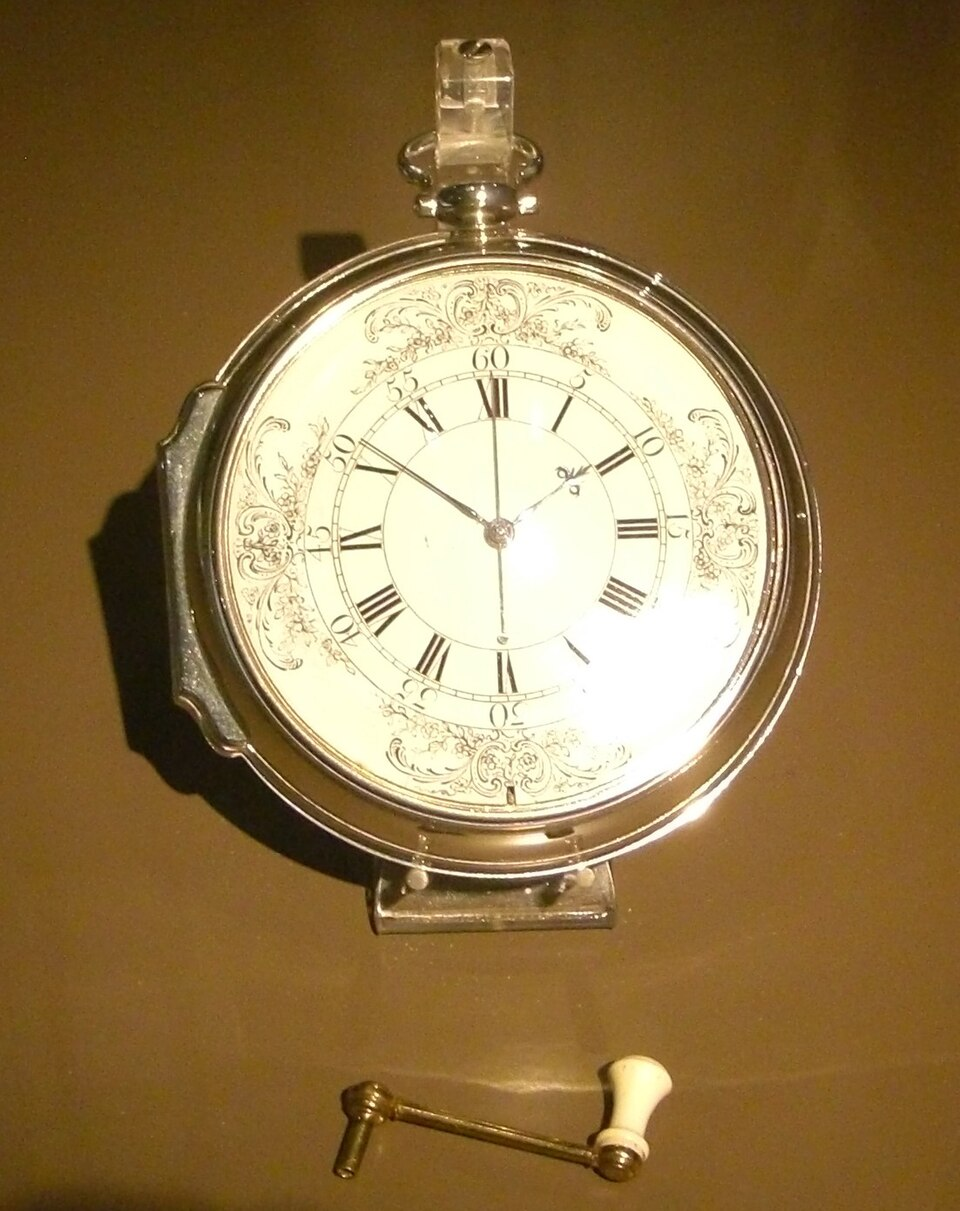
\includegraphics[width=\linewidth]{images/book1/g6-harrison-h4.jpg}\\[2pt]
{\footnotesize El H4 de Harrison, National Maritime Museum, Greenwich.
(Foto: Colonel Warden, CC BY-SA 3.0, vía Wikimedia Commons.)}
% ledger: commons:harrison-h4
\end{minipage}
\end{history}

\section{Ejercicios}

\begin{exercise}[$\star$]\label{exo:g6:latitude-longitude:1}
Copia y completa: ``La \omterm{def:g6:latitude-longitude:latitude}{latitud} se mide desde el \ldots{} y va de $0^\circ$
a \ldots; la \omterm{def:g6:latitude-longitude:longitude}{longitud} se mide desde el \omterm{def:g6:latitude-longitude:longitude}{meridiano} de \ldots{} y va de
$0^\circ$ a \ldots''
\end{exercise}

\begin{exercise}[$\star$]\label{exo:g6:latitude-longitude:2}
¿Cuál es la \omterm{def:g6:latitude-longitude:latitude}{latitud} del \omterm{def:g3:continents-and-oceans:poles}{Polo Norte}? ¿Y la del \omterm{def:g3:continents-and-oceans:poles}{Polo Sur}? ¿Y la de una ciudad
situada en el \omterm{def:g3:continents-and-oceans:equator}{ecuador}?
\end{exercise}

\begin{exercise}[$\star$]\label{exo:g6:latitude-longitude:3}
Usa el \omterm{def:g2:drawing-to-map:map}{mapa} de las trece ciudades para decir en qué \omterm{def:g3:continents-and-oceans:equator}{hemisferio}, norte o
sur, y a qué lado del \omterm{def:g6:latitude-longitude:longitude}{meridiano de origen}, este u oeste, está cada una de
estas ciudades: Sídney, Nueva York, El Cairo, Río de Janeiro.
\end{exercise}

\begin{exercise}[$\star$]\label{exo:g6:latitude-longitude:4}
¿Verdadero o falso? Corrige las frases falsas.
(a) Todos los \omterm{def:g6:latitude-longitude:longitude}{meridianos} se juntan en los \omterm{def:g3:continents-and-oceans:poles}{polos}.
(b) Todos los \omterm{def:g6:latitude-longitude:latitude}{paralelos} tienen la misma \omterm{def:g6:latitude-longitude:longitude}{longitud}.
(c) El \omterm{def:g3:continents-and-oceans:equator}{ecuador} es un \omterm{def:g6:latitude-longitude:latitude}{paralelo}.
(d) El \omterm{def:g6:latitude-longitude:longitude}{meridiano de origen} pasa por París.
\end{exercise}

\begin{exercise}[$\star\star$]\label{exo:g6:latitude-longitude:5}
Usa el \omterm{def:g2:drawing-to-map:map}{mapa} de las trece ciudades: ¿qué ciudad está a unos
$30^\circ$\,N, $31^\circ$\,E? ¿Cuál está a unos $41^\circ$\,N,
$74^\circ$\,O? Da las coordenadas aproximadas de Tokio.
% ledger: data:b1-ne-places (cities.py main table)
\end{exercise}

\begin{exercise}[$\star\star$]\label{exo:g6:latitude-longitude:6}
La ciudad~A está en la \omterm{def:g6:latitude-longitude:longitude}{longitud} $0^\circ$ y la ciudad~B en la \omterm{def:g6:latitude-longitude:longitude}{longitud}
$45^\circ$\,E. ¿Cuántas horas separan sus mediodías? ¿En qué ciudad es
mediodía primero?
\end{exercise}

\begin{exercise}[$\star\star$]\label{exo:g6:latitude-longitude:7}
Bombay está a unos $73^\circ$\,E. Calcula su \omterm{def:g6:latitude-longitude:time-zone}{huso horario} ideal. Cuando es
mediodía en Greenwich, ¿qué hora es en Bombay, en los husos ideales?
% ledger: data:b1-ne-places (cities.py: 72.88 E, zone +5)
\end{exercise}

\begin{exercise}[$\star\star$]\label{exo:g6:latitude-longitude:8}
Cada grado de \omterm{def:g6:latitude-longitude:latitude}{latitud} mide unos \qty{111}{km}. ¿A qué distancia del \omterm{def:g3:continents-and-oceans:equator}{ecuador}
está una ciudad situada a $30^\circ$\,N, medida a lo largo de su \omterm{def:g6:latitude-longitude:longitude}{meridiano}?
¿A qué distancia está el \omterm{def:g3:continents-and-oceans:poles}{Polo Norte} del \omterm{def:g3:continents-and-oceans:equator}{ecuador}?
% ledger: rmg:latitude-def
\end{exercise}

\begin{exercise}[$\star\star$]\label{exo:g6:latitude-longitude:9}
Nueva York está en el huso $-5$ y Tokio en el huso $+9$. ¿Cuántas horas de
diferencia hay entre sus relojes? Cuando son las 8 de la mañana del lunes
en Nueva York, ¿qué hora y qué día es en Tokio?
% ledger: data:b1-ne-places (cities.py: zones -5 and +9)
\end{exercise}

\begin{exercise}[$\star\star$]\label{exo:g6:latitude-longitude:10}
Lena dice: ``El Sol sale por el este, así que las ciudades del este ven
salir el Sol antes que las ciudades del oeste''. ¿Tiene razón? Explícalo
con el giro de la Tierra.
\end{exercise}

\begin{exercise}[$\star\star\star$]\label{exo:g6:latitude-longitude:11}
El reloj de un barco adelanta 3~segundos al día (va demasiado deprisa).
(a) ¿Cuántos segundos va adelantado después de un viaje de 42~días? (b) La
Tierra gira un grado en 4~minutos, es decir, en 240~segundos. ¿Qué error,
en grados de \omterm{def:g6:latitude-longitude:longitude}{longitud}, produce el error del reloj? (c) En el \omterm{def:g3:continents-and-oceans:equator}{ecuador}, un
grado de \omterm{def:g6:latitude-longitude:longitude}{longitud} mide unos \qty{111}{km}. ¿Por cuántos kilómetros se
equivoca, más o menos, el navegante en el \omterm{def:g3:continents-and-oceans:equator}{ecuador}?
% ledger: rmg:longitude-act-1714, rmg:15deg-per-hour, rmg:latitude-def
\end{exercise}

\begin{exercise}[$\star\star\star$]\label{exo:g6:latitude-longitude:12}
Un avión sale de Tokio (huso $+9$) a las 6 de la tarde del lunes y vuela
hacia el este, cruzando el Pacífico, hasta Los Ángeles (huso $-8$). El vuelo
dura 10~horas. (a) ¿Qué hora es en Greenwich cuando sale el avión?
(b) ¿Qué hora es en Greenwich cuando aterriza? (c) ¿Cuál es la hora local
y el día en Los Ángeles cuando aterriza? ¿Por qué dicen los viajeros que en
este vuelo ``aterrizas antes de haber despegado''?
\end{exercise}

\section{Problema: una videollamada alrededor del mundo}

\begin{problem}[{Problema de fin de semana --- cinco amigos, cuatro husos
horarios y una línea de cambio de fecha: ¿qué hora es en Auckland cuando
empieza la llamada?}]
\label{pb:g6:latitude-longitude:1}
% ledger: data:b1-ne-places, rmg:15deg-per-hour, planet:Earth.day (cities.py, time_zones.py; test_cities_zones_used_in_the_problem)
Lena vive en Londres. Quiere organizar una videollamada con cuatro amigos
que conoció en vacaciones: Ana, en Río de Janeiro; Kenji, en Tokio; Mia, en
Auckland; y Sam, en Los Ángeles. En este problema usamos los \omterm{def:g6:latitude-longitude:time-zone}{husos horarios}
ideales.

\begin{center}
\small
\begin{tabular}{lll}
\hline
amigo & ciudad & coordenadas\\
\hline
Lena & Londres & $52^\circ$\,N, $0^\circ$\\
Ana & Río de Janeiro & $23^\circ$\,S, $43^\circ$\,O\\
Kenji & Tokio & $36^\circ$\,N, $140^\circ$\,E\\
Mia & Auckland & $37^\circ$\,S, $175^\circ$\,E\\
Sam & Los Ángeles & $34^\circ$\,N, $118^\circ$\,O\\
\hline
\end{tabular}
\end{center}

\medskip
\noindent\textbf{Parte I --- Dónde viven los amigos.}
\begin{enumerate}
  \item ¿Qué amigos viven en el \omterm{def:g3:continents-and-oceans:equator}{hemisferio sur}?
  \item ¿Qué amigos viven al oeste del \omterm{def:g6:latitude-longitude:longitude}{meridiano de origen}?
  \item ¿Qué amigo vive más lejos del \omterm{def:g3:continents-and-oceans:equator}{ecuador}?
  \item ¿Qué amigo vive más cerca del \omterm{def:g6:latitude-longitude:longitude}{meridiano} $180^\circ$? ¿A cuántos
        grados de \omterm{def:g6:latitude-longitude:longitude}{longitud} de él?
\end{enumerate}

\medskip
\noindent\textbf{Parte II --- ¿Qué hora es?}
\begin{enumerate}[resume]
  \item ¿Cuántos grados gira la Tierra en una hora?
  \item Calcula el \omterm{def:g6:latitude-longitude:time-zone}{huso horario} ideal de la ciudad de cada amigo.
  \item Lena propone empezar la llamada el viernes a las 8 de la tarde,
        hora de Londres. ¿Qué hora y qué día es entonces en Río de Janeiro?
        ¿Y en Tokio?
  \item Kenji contesta que estará dormido. Explica por qué en Tokio ya es
        sábado.
\end{enumerate}

\medskip
\noindent\textbf{Parte III --- Cruzar la línea de cambio de fecha.}
\begin{enumerate}[resume]
  \item ¿Qué hora y qué día es en Los Ángeles cuando empieza la llamada?
  \item ¿Cuántas horas van adelantados los relojes de Auckland respecto a
        los de Los Ángeles?
  \item Navegando hacia el este, de Auckland a Los Ángeles, un barco cruza
        la \omterm{def:g6:latitude-longitude:date-line}{línea de cambio de fecha}. ¿Pasa al día siguiente o vuelve al día
        anterior?
  \item ¿Cuál es la hora local, y el día, en Auckland cuando empieza la
        llamada?
\end{enumerate}
\end{problem}
